% THIS IS SIGPROC-SP.TEX - VERSION 3.1
% WORKS WITH V3.2SP OF ACM_PROC_ARTICLE-SP.CLS
% APRIL 2009
%
% It is an example file showing how to use the 'acm_proc_article-sp.cls' V3.2SP
% LaTeX2e document class file for Conference Proceedings submissions.
% ----------------------------------------------------------------------------------------------------------------
% This .tex file (and associated .cls V3.2SP) *DOES NOT* produce:
%       1) The Permission Statement
%       2) The Conference (location) Info information
%       3) The Copyright Line with ACM data
%       4) Page numbering
% ---------------------------------------------------------------------------------------------------------------
% It is an example which *does* use the .bib file (from which the .bbl file
% is produced).
% REMEMBER HOWEVER: After having produced the .bbl file,
% and prior to final submission,
% you need to 'insert'  your .bbl file into your source .tex file so as to provide
% ONE 'self-contained' source file.
%
% Questions regarding SIGS should be sent to
% Adrienne Griscti ---> griscti@acm.org
%
% Questions/suggestions regarding the guidelines, .tex and .cls files, etc. to
% Gerald Murray ---> murray@hq.acm.org
%
% For tracking purposes - this is V3.1SP - APRIL 2009

\documentclass{acm_proc_article-sp}
\usepackage{url}

%
\def\sharedaffiliation{%
\end{tabular}
\begin{tabular}{c}}
%

\begin{document}


\title{Similar Article Detection Using Minhash Technique on Wikipedia\titlenote{This effort is part of the CMSC828G, Data Intensive Computing with MapReduce, class project.}}
%
% You need the command \numberofauthors to handle the 'placement
% and alignment' of the authors beneath the title.
%
% For aesthetic reasons, we recommend 'three authors at a time'
% i.e. three 'name/affiliation blocks' be placed beneath the title.
%
% NOTE: You are NOT restricted in how many 'rows' of
% "name/affiliations" may appear. We just ask that you restrict
% the number of 'columns' to three.
%
% Because of the available 'opening page real-estate'
% we ask you to refrain from putting more than six authors
% (two rows with three columns) beneath the article title.
% More than six makes the first-page appear very cluttered indeed.
%
% Use the \alignauthor commands to handle the names
% and affiliations for an 'aesthetic maximum' of six authors.
% Add names, affiliations, addresses for
% the seventh etc. author(s) as the argument for the
% \additionalauthors command.
% These 'additional authors' will be output/set for you
% without further effort on your part as the last section in
% the body of your article BEFORE References or any Appendices.

\numberofauthors{5} %  in this sample file, there are a *total*
% of EIGHT authors. SIX appear on the 'first-page' (for formatting
% reasons) and the remaining two appear in the \additionalauthors section.
%
\author{
% You can go ahead and credit any number of authors here,
% e.g. one 'row of three' or two rows (consisting of one row of three
% and a second row of one, two or three).
%
% The command \alignauthor (no curly braces needed) should
% precede each author name, affiliation/snail-mail address and
% e-mail address. Additionally, tag each line of
% affiliation/address with \affaddr, and tag the
% e-mail address with \email.
%
% 1st. author
\alignauthor Samet Ayhan\\
       \affaddr{University of Maryland, Department of Computer Science}\\
       \affaddr{College Park, Maryland 20740}\\
       \email{sayhan@cs.umd.edu}
% 2nd. author
\alignauthor Joshua Bradley\\
       \affaddr{University of Maryland, Department of Computer Science}\\
       \affaddr{College Park, Maryland 20740}\\
       \email{jgbradley@cs.umd.edu}
% 3rd. author
\alignauthor Sarah Weissman\\
       \affaddr{University of Maryland, College of Information Studies}\\
       \affaddr{College Park, Maryland 20740}\\
       \email{sweissman@umd.edu}
}
% There's nothing stopping you putting the seventh, eighth, etc.
% author on the opening page (as the 'third row') but we ask,
% for aesthetic reasons that you place these 'additional authors'
% in the \additional authors block, viz.

\date{19 April 2013}
% Just remember to make sure that the TOTAL number of authors
% is the number that will appear on the first page PLUS the
% number that will appear in the \additionalauthors section.


\maketitle
\begin{abstract}
In this paper, we describe a novel similarity detection algorithm that utilizes locality sensitive hashing technique on MapReduce framework. The algorithm has been designed and implemented to detect similar articles using large Wikipedia dumps, in compressed or uncompressed forms.
\end{abstract}

% A category with the (minimum) three required fields
\category{H.2.4}{Information Systems}{Database Management}[Systems]

\terms{Algorithms, Design, Performance}

\keywords{Big Data, Data Analytics, Data Warehouse, Data Stream Management} % NOT required for Proceedings

\section{Introduction}
Wikipedia has a history of generating controversy over editorial quality and factual correctness. Although some studies have found Wikipedia’s accuracy to rival that of traditional encyclopedias, other studies have found numerous factual errors [1]. Since Wikipedia may be edited anonymously, information is often freely copied between web sources or other Wikipedia articles. Additionally, many articles in Wikipedia lack citations. There is little mechanism for detecting and correcting such errors. One potential source of error on Wikipedia is factual information that varies over time and is not updated. Wilkinson found that the distribution of article edits has a long tail, meaning that a small number of articles have many edits while most articles have few, and that number of edits is directly related to article quality. Articles with low edits, and low editorial attention, are less likely to be updated when new information becomes available \cite{wilkinson:wiki}.

As a step toward identifying factual errors, we investigated the problem of finding near duplicate sentences on Wikipedia. Such near duplicate sentences may reflect factual information that has been updated in one article and not another, or merely inconsistencies that should be flagged and addressed. We used the MapReduce computing framework and locality sensitive hashing techniques to compare sentences and identify near duplicates.

The rest of this paper is organized as follows: In Section 2, we present related work, in Section 3, we explain the algorithm utilizing locality sensitive hashing, in Section 4, we present the working application within MapReduce framework. In Section 5, we discuss our experiments with various Wikipedia datasets. The final section contains concluding remarks and future work.

\section{Related Work}
A number of techniques have been implemented to identify similarity between documents in the literature. These techniques usually differ in terms of corpus of interest, signature representing the document, feature-set determined by the system, and the end goal. In addition to these differences, one can also consider the efficiency and scalability of the system, overall. 

In this section, we will go over some of theses techniques offered in the literature. Additionally, we will highlight our novel contribution.

Broder et al. introduced shingling to compute document similarity and containment. They also presented methods for using a subset of shingles while still allowing similarity and containment computations \cite{broder:resemblance}.

Seo et al. defined a general framework for text reuse detection. They introduced Discrete Cosine Transform (DCT) fingerprinting for general or local text reuse detection with high accuracy and efficiency \cite{seo:dct}.

Zhang et al. presented partial duplicate detection algorithm using sequence matching that transforms partial-duplicate detection task into three MapReduce jobs: 1.Indexing, 2.Sequence Duplicate Detection, 3.Sequence Matching \cite{zhang:pdc}.

Hajishirzi et al. introduced an adaptive near-duplicate detection (ANDD) method by extending term-weighting framework to learn k-gram vectors. Provided that each document was represented by an informative real k-gram vector, similarity measures were computed to come up with predicted values of near-duplicates \cite{hajishirzi:andd}.

Lin described three MapReduce algorithms for computing pairwise similarity on document collections: 1.Based on brute force, 2.Treated as large-scale ad hoc retrieval, 3.Based on Cartesian product of postings lists \cite{lin:brute}.

Manku et al. used Charikar's fingerprinting technique for developing near-duplicate detection system. They presented an algorithmic technique for identifying existing f-bit fingerprints that differ from a given fingerprint in at most k bit-positions, for small k. They demonstrated that their system is useful not only for batch but also for online processing \cite{manku:web}.

Bendersky et al. examined two information flow representations: the timeline and the link graph. They proposed several simple unsupervised techniques for timeline construction link graph analysis \cite{bendersky:timeline}.

In order to handle large Wikipedia dumps with the order of tens or hundreds of gigabytes and even a few terabytes, we used MapReduce framework in this work, that was introduced by Dean and Ghemawat \cite{dean:mapreduce}. The implementation is able to stream the compressed bz2 dumps and feed into mappers and reducers for further processing, which will be detailed in the following sections.

\section{Algorithm Utilizing Locality Sensitive Hashing}
In this section, we introduce the algorithm that utilizes the locality sensitive hashing.

\subsection{Design}
We explain the design here...

\subsection{Implementation}
We explain the implementation here...

\section{Working Application}
We explain the working application here...

\begin{figure}
\centering
\epsfig{file=figure1.eps,height=1in,width=2.2in}
\caption{Workflow within MapReduce Framework.}
\end{figure}

\section{Experiments and Discussion}
In this section, we discuss some of the issues we encountered regarding data representation, and archived data loading. We also present the performance optimizations we realized.

\subsection{Optimizations}	 
We explain optimizations here...

\subsubsection{Optimization-1}
An optimization we realized...

\subsubsection{Optimization-2}
Another optimization we realized...

\begin{figure*}
\centering
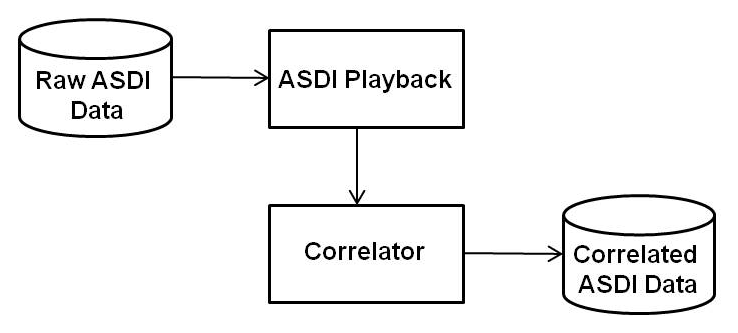
\epsfig{file=figure2.eps,height=1.5in,width=7in}
\caption{Some figure.}
\end{figure*}

Illustrated in Figure 2, explain the figure here...

\section{Conclusion and Future Work}
Conclusion goes here...


\section{Acknowledgments}
We would like to thank all of the anonymous contributors. We would especially like to thank Jimmy Lin for his advise and directions.

%
% The following two commands are all you need in the
% initial runs of your .tex file to
% produce the bibliography for the citations in your paper.
\bibliographystyle{abbrv}
\bibliography{sigproc}  % sigproc.bib is the name of the Bibliography in this case
% You must have a proper ".bib" file
%  and remember to run:
% latex bibtex latex latex
% to resolve all references
%
% ACM needs 'a single self-contained file'!
%
%APPENDICES are optional
%\balancecolumns
\balancecolumns
% That's all folks!
\end{document}
